\subsection{Abstract Syntax Trees}
\begin{frame}{Abstract Syntax Trees}
    ASTs represent the abstract syntax of a program.
    Abstract means that unnecessary tokens are removed, ex. parenthesis, curly braces.\\
    It's produced by the Syntax Analyzer.\\
    Often used as an intermediary representation by the interpreter.
\end{frame}

\subsection*{Sum of Products}
\begin{frame}[fragile]{Sum of Products}
    \begin{lstlisting}[language=Haskell]
        data SomeType = A Bool Bool Bool
                        | B Bool
                        | C
    \end{lstlisting}
\end{frame}

\begin{frame}{Sum of Products}
    \begin{equation*}
        \underbrace{(\text{Bool} \times \text{Bool} \times \text{Bool})}_{A} + \underbrace{\text{Bool}}_{B} + \underbrace{1}_{C}
    \end{equation*}
    The Bool type can take on 2 different values (True or False ), so the A constructor can construct $2 * 2 * 2 = 8$ different values.\\
    the total numbers of values of type SomeType is $8 + 2 + 1 = 11$, as the data type is the sum of the three products we've just described.
\end{frame}

\subsection{Static Analysis}
\subsubsection*{Type Checking}
\begin{frame}{Type Checking}
    Typing falls into two categories
    \begin{itemize}[<+->]
        \item Static
        \item Dynamic
    \end{itemize}
\end{frame}

\begin{frame}{Type Checking}
    Example!

\end{frame}

\subsubsection*{Wellformedness}
\begin{frame}{Wellformedness}
    For a program to be Wellformedit needs to satisfy all the constraints(kinda like rules) on it. This
    means that the program follows all the rules for it like;
    \begin{itemize}
        \item The program conforms to the AST
        \item Typed correctly
        \item all procs/declarations are wellformed
        \item other things
    \end{itemize}
\end{frame}

\subsubsection*{Type Inference}
\begin{frame}{Type Inference}
    Some languages don't specify the type of expressions and therefore need to be inferred.
    Example!
\end{frame}

\subsection*{Q\&A}
\begin{frame}{Questions?}
    \begin{figure}
        \centering
        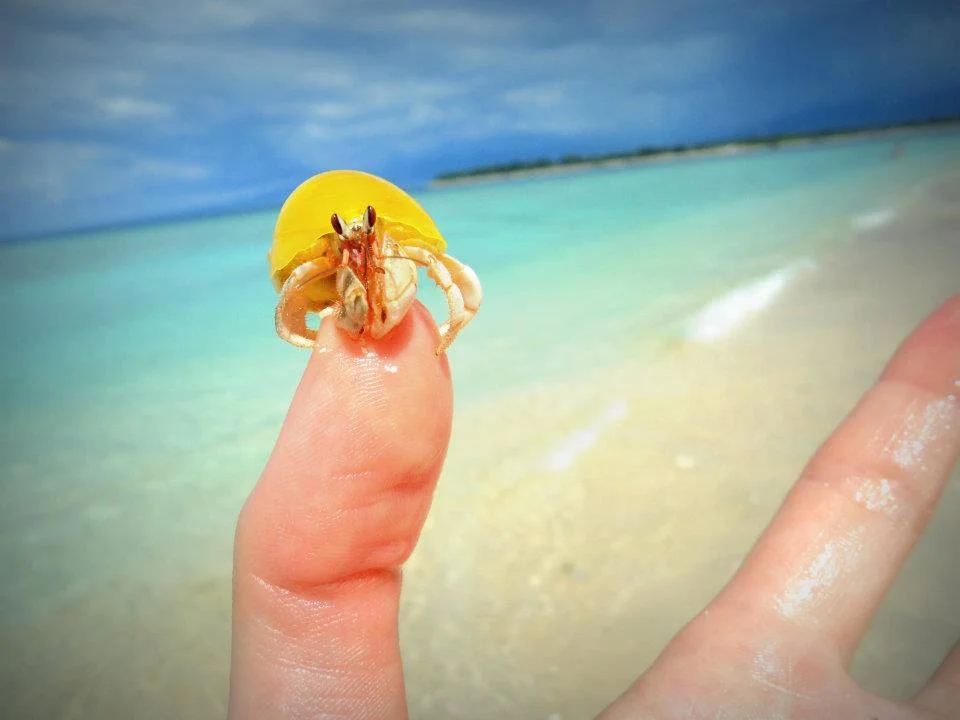
\includegraphics[height = 4.9cm]{intermission/chap03.png}
    \end{figure}
\end{frame}